\chapter{Neutrinoforschung}
\vspace{8pt}

\section{Das Neutrino}
Das Neutrino ist ein subatomares Teilchen der Leptonenklasse. Das Neutrino hat keine
elektrische Ladung und unterliegt somit nur der schwachen Wechselwirkung und der
Massenanziehungkraft. Nach dem Standardmodell ist das Neutrino ein punktförmiges Teilchen.
Es gibt 3 Generationen von Neutrinos mit jeweils anderer Masse.
Da Neutrinos ein Spin von $\frac{1}{2}$ haben, sind sie Fermionen. \\ \cite{Stoecker2000}
\begin{center}
    \begin{tabular}{ | l | c | } \hline
        Bezeichnung & Masse (MeV) \\ \hline
        Elektron-Neutrino & >7,3 $\cdot 10^{-6}$\\
        Muon-Neutrino & <0,27  \\
        Tau-Neutrino & <31 \\ \hline
    \end{tabular}
\end{center}
Die Masse wurde bis dato nicht genau bestimmt,
aber es wurden bisher Obergrenzen bestimmt.\\
Kosmische, solare, atmosphärische oder Geoneutrinos entstammen aus natürlichen Quellen bzw.
natürlichen Reaktionen.
Reaktorneutrinos und Beschleunigerneutrinos entstammen aus künstlichen Quellen bzw. künstlichen
Reaktionen. \\
Neutrinos können bei der Überprüfung der Plutoniumproduktion von Kernkraftwerken eingesetzt
werden, indem man die Antineutrinoemissionen misst. \cite{Krauter2006} \\
Insbesonders in der Astrophysik sind Neutrinos von hoher Bedeutung.
Da sie nur schwach wechselwirken durchdringen sie fast jede Materie und so kann man durch
Neutrinos Weltraumregionen untersuchen, die sonst aufgrund von Strahlungseinflüssen
nicht untersucht werden könnten.
Zudem ist die Masse von Neutrinos bedeutend für viele astrophysikalische Theorien. 

\subsection{Symmetrie}

\subsubsection{Händigkeit}

Es ist wichtig zwischen Chiralität und Helizität zu unterscheiden.
Die beiden Konzepte werden gerne vertauscht, da beide oft durch rechts und links ausgedrückt werden.
Die Helizität ist abhängig von der Drehrichtung eines Teilchens und des Spins eines Teilchen. \cite{Gold1958}
Die Helizität ist bei massereichen Teilchen vom Bezugssystem abhängig und bei masselosen Teilchen fest
definiert. Die Chiralität ist immer unabhängig vom Bezugssystem, ist also eine Lorentz-Invariante.
Bei masselosen Teilchen ist die Chiralität gleich der Helizität.\\
Nach bisherigen Versuchen haben Neutrinos eine negative Helizität (linkshändig) und seine
Antiteilchen eine positive Helizität (rechtshändig).
Auch wurde festgestellt, dass deren Helizität und Chiralität sich gleichen. Also könnte man davon ausgehen, dass
das Neutrinos masselos ist. \\
Dies steht natürlich im Widerspruch mit der Tatsache, dass Neutrinos eine Masse haben.
Dies ist auch im Moment noch ein offene Frage. Auch das IceCube-Projekt beschäftigt sich mit dieser Frage.
Eine mögliche Lösung wäre, dass das Neutrino wie andere Teilchen eine rechtshändige und linkshändige Version hat.
Ein rechtshändiger Neutrino würde nicht schwach wechselwirken, diese Neutrinos bezeichnet man als steriles
Neutrino. Man hofft, dass ein bestimmtes Mechanismus zwischen dem aktiven und sterilen Neutrino sowohl deren Masse
als auch die Symmetrien erklärt.

\subsubsection{Leptonenladung}

Das Neutrino hat ein positve Leptonenladung, während das Antineutrino eine negative Leptonenladung hat. Also kann man
zwischen Teilchen und Antiteilchen differenzieren, da sie verschiedene Quantenzahlen haben.\cite{Stoecker2000}
Diese Unterscheidung gibt es aktuell aber nur nach dem Standardmodell. Das zuvor erwähnte Mechanismus wird als See-Saw-Mechanismus
bezeichnet, dieses erfordet sogenannte Majorana-Spinoren, also im Grunde müsste die Leptonenladung von Neutrino und
Antineutrino gleich sein. Bis dato konnte man nicht experimentell bestimmen ob Neutrino und Antineutrino sich wirklich
unterscheiden.

\subsection{Geschwindigkeit und Masse}

Neutrinos haben nach momentanen Verständnis eine Masse. Nach dieser Annahme dürften Neutrinos nicht mit Lichtgeschwindigkeit
sich fortbewegen können. Nach der speziellen Relativitätstheorie gilt folgende Formel:
\begin{center}
    $E={\dfrac {m_0c^{2}}{\sqrt {1-{\frac {v^{2}}{c^{2}}}}}}$ \cite{Stoecker2000}
\end{center}
Würde ein Teilchen sowohl eine Ruhemasse $m_0 > 0$, als auch sich mit einer Geschwindigkeit $v=c$ fortbewegen,
dann würde sich eine Definitionslücke ergeben, da $x/0$ nicht definierbar ist.
\begin{center}
    $E={\dfrac {m_0c^{2}}{0}} $
\end{center}
Da die Annahme $m_0 > 0$ und $v=c$ nach der speziellen Relativitätstheorie keine Definition über die Energie des Teilchen
bei Bewegung zu lässt geht man davon aus die Annahme sei falsch.
Also bleiben nach der Theorie 2 mögliche Lösungen übrig. Entweder hat das Neutrino doch keine Ruhemasse, also es gibt
irgendein bisher nicht bekannten Masseeffekt oder das Neutrino bewegt sich nur subluminar.

\subsubsection{Erste Untersuchungen}

Eine erste Untersuchung der Geschwindigkeit von Neutrinos war ein Versuch von FermiLab in den 70ern.
Man konnte mit hoher Konfidenz feststellen, dass sich Neutrinos mit Lichtgeschwindigkeit fortbewegen.
Bei der Supernova SN1987A hat man diese Festellung nochmal bestätigt. Die Geschwindigkeit von $\overline{\nu}_e$
hat maximal ein Abweichung von $2x10^{-9}$ zur Lichtgeschwindigkeit. \cite{Longo1987}

\subsubsection{OPERA-Experiment}

Andere Messungen haben dies weiter bestätigt. Das OPERA-Experiment hat im Zeitraum von 2009-2011 Messungen bezüglich der Geschwindigkeit von Neutrinos
durchgeführt. Es wurde festgestellt, dass Neutrinos sich superluminal bewegen. Auf einem Weg von 743km kamen die Neutrinos
$60,7 \pm 14,3 ns$ früher an als wenn sie sich mit Lichtgeschwindigkeit fortbewegen würden. Mit einer $6\sigma$-Sicherheit
konnte man von einen sehr signifikaten Ergebnis reden. Diese Messungen wurden am 22.September 2011 in
einem Vordruckserver veröffentlicht. \cite{OPERA2011} \\
Im nächsten Jahr wurde dies aber korrigiert. Man hatte festgestellt, dass eine Kabelverbindung die gemessen Geschwindigkeiten
verändert hat. Es ergab sich nur eine Abweichung von $6.5_{-15.4}^{+15.7}\, ns$. In der weiteren Analyse kam man
zum Schluss, dass die Ergebnisse die Tatsache bestätigen, dass Neutrinos sich mit Lichtgeschwindigkeit bewegen.
Eine letzte Annahme könnte sein, dass zwar nach bisherigen Messungen Neutrinos sich mit großer Sicherheit mit
Lichtgeschwindigkeit fortbewegen, aber dies nur der Fall ist, weil deren Masse so gering ist, dass die Abweichung
zur Lichtgeschwindigkeit zu gering ist um sie messen zu können. Sie müsste kleiner als $2x10^{-9}$ sein.

\section{Geschichte}

\subsection{$\beta^{-}$ Zerfall}

Beim $\beta^{-}$-Zerfall gibt es folgende Reaktion:
\begin{center}
$n \rightarrow p + e^- + \overline{\nu}_e$
\end{center}
Vor der Entdeckung des Neutrino, hat man beim $\beta^{-}$-Zerfall nur die folgende Reaktion beobachtet:
\begin{center}
$n \rightarrow p + e^-$
\end{center}
Nimmt man diese Beobachtung kommt man auf den Energiehaltungssatz:
\begin{center}
$ E_e = E_n - E_p $
\end{center}
Man geht davon aus, dass das Neutron kein Impuls hat aufgrund der Laborbedingungen, also folgt
$p_n = 0$. \\
Aufgrund der Impulserhaltung ergibt sich folgendes:
\begin{center}
$ - p_e = p_{He} $
\end{center}
So kommt man zur Formel zur Berechnung der Energie des Elektrons:
\begin{center}
$ E_e = c^2 \frac{m_H^2 - m_{He}^2+m_e^2}{2m_H} $
\end{center}
$E_e$ beträgt somit $18,7 keV$. \\
Die gesamte Herleitung ist in der Quelle \cite{Horak2015} zu finden. \\ \\
Der entsprenchende Versuch lieferte jedoch nicht ein Linienspektrum für die Elektronenenergie,
man schlussfolgert also, dass die Elektronenenergie nicht konstant ist.
Man stellte jedoch fest, dass die höchste Elektronenenergie des Spektrum der Berechneten gleicht.
Aufgrund des Energieerhaltungssatz muss die restliche Energie irgendwie umgewandelt werden.
\cite{Horak2015} (siehe Anhang \ref{fig:b-zerfall}) \\ \\
Die erste mit dem Energieerhaltungssatz konforme Erklärung für dieses Phänomen kam mit einem Brief von
Pauli an die Teilnehmer der Gauverein-Tagung in Tübingen.
Im Brief postuliert er, dass dieses Energiespektrum aufgrund eines weiteren Teilchen
entsteht. \cite{Pauli1930} \\
Für Jahre konnte man keine Messung durchführen, welche dieses Teilchen beweisen würde.
Das postulierte Teilchen sollte aber elektrisch neutral sein und nur schwach wechselwirken.

\subsection{Reines-Cowan-Experiment}

Das postulierte Neutrino sollte in einem umgekehrten $\beta^{-}$-Zerfall mit einem Proton interagieren
und einen Elektron und Positron erzeugen.
\begin{center}
$\overline{\nu}_e + p \rightarrow e^+ + n$
\end{center}
Diese Reaktion hat ein Wirkungsquerschnitt $6 x 10^{-44} cm^2$, dieser ist 20 Magnituden kleiner ist als die entsprechende
Standardeinheit Barn ($10^{-24} cm^2$).
Durch den sehr kleinen Wirkungsquerschnitt ist die Reaktion sehr selten, also musste sie einfach identifizierbar
sein, da man nicht die wenigen Ereignisse verpassen wollte.
Die zwei Zerfallsprodukte sind Positronen und Neutronen. Die Positronen lässt man mit Elektronen interagieren
und so werden 2 Cadmiumen emittiert.
Diese 2 $\gamma$-Strahlen würden nicht reichen um die Reaktion leicht zu identifizieren.
Also lässt man noch das Neutron mit $Cd^{108}$ interagieren. Trifft ein Neutron auf $Cd^{108}$, regt es dieses an.
Diese angeregte Zustand ist instabil und das Cadmium gibt die Energie als $\gamma$-Strahlung frei. Dieser Prozess
passiert nicht sofort, also hat es eine Zeitsignatur.
Durch diese Kombination aus 2 $\gamma$-Strahlen und einem zeitverzögerten $\gamma$-Strahl kann man die Reaktion einfach
identifizieren und ist klar zu erkennen trotz Hintergrundstöreinflüssen. \\
Man benötigte dennoch ein hohen Neutrino Flux um die seltene Reaktion beobachten zu können. Dies konnte
man mit einem Atomreaktor erreichen, dieser sollte ein Neutrino-Flux von  $10^{12}-10^{13}$ Neutrinos
pro Sekunde pro Quadratzentimeter haben. \cite{Nave2017} (Anhang \ref{fig:c-experiment}) \\
Der entsprechende Versuch wurde in Hanford und schließlich in Savannah River durchgeführt, es wurden
durchschnittlich 3 Neutrinos pro Stunde gemessen. Die Ereignissanzahl war größer mit eingeschaltetem
Reaktor. \\
Die Ergebnisse aus dem Versuch legten nahe, dass Pauli mit seiner Neutrino-These korrekt lag.

\subsection{Homestake-Experiment}

In der Sonne gibt es Reaktionen, welche Neutrinos produzieren. 86\% dieser Neutrinos stammen aus der
Proton-Proton-Reaktion.
\begin{center}
$p + p \rightarrow d + e^- + \nu_e$
\end{center}
1968 konnten man den Neutrino-Flux der Sonne messen mit dem Homestake-Experiment.\cite{Cleveland1998}
Es wurde jedoch ein Defizit zwischen den berechneten Flux und den gemessen Flux festgestellt.
Es ist wichtig zu vermerken, das Homestake-Experiment konnte nur Elektron-Neutrinos messen .
Diese Problematik wurde bekannt als das Solarneutrino-Problem. Es wurde zum Beispiel vermutet, dass die Fusionprozesse
temporär ausgesetzt sind oder die Sonne ist kälter als man vermutet hatte. Das passte aber nicht zu den
helioseismologischen Daten, welchen mit dem Standard-Sonnenmodell übereinstimmten.

\subsection{Neutrino-Oszillation}

In den 70ern wurde vermutet, sollten Neutrinos eine Masse haben, dann würden sie zwischen den einzelnen Flavours
wechseln können. \cite{Gribov1969}
Bei den Proton-Proton-Reaktionen, welche in der Sonne stattfinden zerfallen Elektronen-Neutrinos.
Also könnten die fehlenden Neutrinos auf den Weg zur Erde den Flavour gewechselt haben und wären so nicht bei dem
Homestake-Experiment messbar.
2001 wurde das Problem dann endgültig gelöst. Das SNO konnte die Neutrino-Oszillation, also der Wechsel
zwischen einzelnen Neutrino-Flavours, nachweisen. Das Experiment bewies auch,
dass die Oszillation das Defizit von Elektron-Neutrinos erklärt.\cite{Ahmad2001}
Bei der Neutrinooszillation wechselt das Neutrino nach zurückgelegten Weg seinen Flavour.
Das Neutrino hat im Grunde 3 Massen-Eigenzustände $\nu_1,\nu_2,\nu_3$. Jedes der Flavours ist eine bestimmte
Überlagerung dieser 3 Massen-Eigenzuständen. Das Neutrino kann in entweder einem festen Flavour-Zustand sein, also
$\nu_e,\nu_\mu,\nu_\tau$ oder ein festen Massezustand. Mithilfe der Quantemechanik kann man die Eigenzustände als
Wellen betrachten. Also kann mithilfe der Schrödinger-Gleichung betrachten wie sich das Neutrino wandelt über ein
bestimmten Zeitraum.

\section{Forschung}

\subsection{Astrophysik}

Das GZK-Cutoff limiert wie stark energetisch komische Strahlung sein kann.
Der Cutoff wurde bei $6x10^{19} eV$ festgestellt und berechnet. \\
Dies limitiert die Beobachtung von komischer Strahlung bei Objekten die weiter als 100 Megaparsec sind.
Elektromagnetische Strahlung interagiert mit Staub- und Gaswolken, weshalb diese Signale abschirmen können.
Neutrinos jedoch haben kein GZK-Cutoff und interagieren nicht mit Stau- und Gaswolken, weshalb einige
komische Objekte nur mit Neutrinomessungen untersucht werden können. Supernovae setzen ein hohen Anteil
an Neutrinos und somit eignet sich die Beobachtung von Neutrinos für Supernovaeforschung. Das IceCube-Projekt
ist einer der wichtigsten Neutrinodetektoren für kosmische Neutrinos.

\subsection{Kosmologie}

In der Kosmologie ist kosmische Mikrowellenhintergrundstrahlung (3K-Strahlung) sehr wichtig gewesen um viele
Theorien, wie die Urknalltheorie, zu bestätigen. Die 3K-Strahlung entstand ungefähr 380 Tausend Jahre nach dem
Urknall. Es gibt einen entsprenchenden Counterpart mit Neutrinos. Der kosmiche Neutrinohintergrund ist wie die 3K-Strahlung
durch den Urknall entstanden.
Im frühen Beginn des Universums gab es viele Interaktionen zwischen Teilchen. Bei vielen Reaktionen entstehen Lichtquanten
und Neutrinos. Da Neutrinos kaum interagieren, können wir diese noch heute messen.
Die Neutrinos die dort enstanden interagierten nur mit anderen Teilchen in der ersten Sekunde in der das Universum
existierte. So ergibt sich eine Temperatur dieser von nur 1,95K. Umgerechnet liegen die Neutrinos im Energiebereich
von ungefähr $100-200 \mu eV$. Neutrinodetektoren können aber meisten nur ab den MeV-Bereich messen. Also
konnte man dies nicht direkt beweisen. Mit dem Planck-Weltraumteleskop konnte man aber die 3K-Strahlung so genau
messen und untersuchen, dass man über diese indirekt den kosmischen Neutrinohintergrund nachweisen konnte.
Die Messungen von Planck-Satellit war so genau, dass man darüber hinaus beweisen konnten, dass der Hintergrund eine
Temperatur von 1,96K hatte und das es nur 3 Neutrino-Flavours gibt ($e,\mu,\tau$). Die erwähnten Temperaturen
gelten nur unter der Bedingung, dass Neutrinos masselos sind. \cite{Siegel2016} Dies widerspricht aber der Tatsache,
dass nach aktuellen Messungen Neutrinos eine Masse haben. Also ist die Untersuchung des kosmichen Neutrinohintergrund
noch nicht vollendet.

\subsection{Zukünftige Forschung}

Das Neutrino hat durchaus die Teilchenphysik revolutionert und es dürfte auch in der Zukunft neue wichtige
Erkentnisse in der Teilchenphysik liefern. \\
ARIANNA und das Giant Radio Array for Neutrino Detection sollen auch wie das IceCube hochenergetische Neutrinoquellen
finden. Es gibt schon weitere Experimente in diesen Bereich, welche für ein Interesse der wissenschaftliche Gemeinde sprechen. \\
Ein kleiner Forschungzweig untersucht inwiefern man Neutrinos für Kommunikation durch solides Gestein nutzen könnte.
Es wurden auch schon entsprechende Versuche gemacht und man konnte erfolgreich Informationen mithilfe von Neutrinos durch
Gestein senden.

\subsubsection{DUNE}

Eines der großen Neutrinoexperimente die geplant werden ist das DUNE. Damit sollen Neutrinos produziert
und dann durch eine große Entfernung gesendet werden und dann an ein anderen Standort empfangen und gemessen werden.
(Anhang \ref{fig:dune}). \\ Das DUNE Experiment hat sich hohe Ziele gesetzt und will die Entstehung von Materie,
die Verbindung aller fundamentalen Kräfte und die Entstehung von schwarzen Löcher näher erklären.
Diese hohen Ziele haben unter anderem damit zutun, dass die Neutrinos möglicherweise das Standardmodell
durcheinanderbringen könnten. Im Moment hat das Standardmodell nur Dirac-Fermionen, also solche mit unterscheidbaren Antiteilchen.
Möglicherweise existieren jedoch Majorana-Fermionen, welche Antiteilchen haben mit gleichen Eigenschaften, also
kann man die nicht unterscheiden. Es gibt bereits Erweiterungen des Standardmodells mit Majorana-Fermionen, bisher
wurde keine dieser Erweiterungen experimentell bestätigt. \\ Das DUNE-Projekt könnte auch die
Materie-Antimaterie-Diskrepanz des frühen Universums erklären, welche zum heutigen Universum voller Materie
und mit kaum Antimaterie führte.

\section{Forschung am IceCube}

\subsection{Astrophysikalische Forschung}

Das größte Erfolg des IceCube ist bewiesen zu haben, dass mithilfe von Neutrinos man Bereiche des Universums
untersuchen kann, welche zuvor nicht untersuchbar ware, wie in 2.3.2 näher erklärt.
Dazu gehört, dass man 2017 durch die Kollaboration mit anderen Instituten zum ersten Mal
außergalaktische Neutrinos messen konnte. Diese stammten vom Blazar TXS 0506+056 aus der Orion-Konstellation.
Am Detektor wurde ein Alarm ausgelöst, weil man ein hochenergetisches (\textasciitilde 300 TeV) Muon-Neutrino maß. Anschließen
haben andere Institute mit deren Instrumenten nach der Quelle gesucht und diese als TXS 0506+056 identifiziert.
Dieses Ereignis wird insbesondere als Erfolg gewertet, weil damit zum ersten mal das Warnsystem erfolgreich erprobt
wurde. Mittlerweile wurde das Warnsystem erweitert, es gibt ein offenes System für Einzelereignisse und Mehrfachereignisse werden
durch Einzelvereinbarungen verschiedenen Instituten verteilt.
Über die Jahre wurden über 100 hochenergetische Neutrinos gemessen. Die gemessenen Energien ging von 100 TeV bis 10 PeV.
Die hochenergetischen Neutrinos scheinen zudem ein hohen Neutrino-Flux mit sich zu bringen.
\cite{WiMa2018}

\subsubsection{Gammastrahlenausbrüche}

Es wird vermutet, dass Gammastrahlenausbrüche die bisher gemesse hochenergetische kosmische Strahlung erklärt. Zudem wird auch
vermutet, dass Gammastrahlenausbrüche auch die hochenergetischen Neutrino-Events auslösen.
Das IceCube untersucht auch dies, da es in der Lage ist in den benötigten Energiebereich Neutrinos zu messen.
Bei diesen Gammastrahlenausbrüche kollidieren hochenergetische Protonen miteinander, also entstehen Pionen. \cite{Abbasi2011}
\begin{center}
$\,\pi ^{+}\to \mu ^{+}+\nu _{{\mu }} \;\;|\;\; \,\pi ^{-}\to \mu ^{-}+\overline {\nu }_{{\mu }}$ \\

$\pi ^{0}\to 2\gamma $
\end{center}
Geladene Pionen zerfallen unter anderem in Myon-Neutrinos und die neutralen Pionen in $\gamma$-Strahlen. Es ist naheliegend, dass
hochenergetische Neutrinos und hochenergetische $\gamma$-Strahlen aus den selben Quellen stammen \cite{Mueller2014}

\subsubsection{Supernovae}

Das IceCube-Projekt war zunächst nicht dafür gedacht Supernovae zu beobachten, da die Neutrinos, die bei einer Supernovae ausgestoßen werden
zu niederenergetisch sind damit das IceCube-Detektor sie messen kann. Doch die Photomultiplier müssten bei niederenergetischen Neutrinos
aus einem Supernovae-Ereignis kollektiv eine höhere Hintergrundrate aufweisen. Bei einer Supernova wird 99\% der Gravitationsenergie
als Neutrinos freigegeben, also entsteht ein hoher Neutrino-Flux.
Sollte ein Erhöhung der Hintergrundrate festgestellt werden wird das direkt an das Supernova Early
Warning System weitergegeben, damit andere Institute nach der Supernova suchen und möglicherweise mehr Daten sammlen. \cite{Eberhardt2017}

\subsubsection{Dunkle Materie}

Eines der größten Fragen der Astrophysik ist was ist Dunkle Materie. Auch hier gibt es entsprechende Versuche mit dem IceCube.
Eine möglicher Kandidat für dunkle Materie sind WIMP-Teilchen. WIMP's interagieren nur durch die schwache Wechselwirkung und der Gravitation.
Anders als Neutrinos sind sie jedoch sehr massereich. \cite{Gaensler2008}
Da WIMP's nur schwach wechselwirken sind sie auch schwer nachzuweisen.
Eine möglicher WIMP-Kandidat das Kaluza-Klein-Teilchen würde sich in Gestirnen ansammlen und wenn die Dichte hoch genug ist
würde sich selber annihilieren. Eines der Zerfallsprodukte wären Neutrinos im GeV/TeV Bereich.
Also würde eine erhöhte Anzahl an Neutrinos aus der Sonne nahelegen, dass das Kaluza-Klein-Teilchen
möglicherweise existiert. \cite{Abbasi2010}

\subsection{Glaziologie}

Das IceCube-Projekt fokusiert sich hauptsächlich auf Physik, durch seine besondere Lage im Eis des Südpol wurde es
auch für glaziologische Untersuchungen benutzt.
Das Eis, welches die optischen Sensoren des IceCube-Detektor umgibt, ist nicht 100\% durchsichtig, da es Impuritäten hat
wie zum Beispiel Staub. Die Daten von den optischen Sensoren müssen entsprechend korrigiert werden. Dieser Staub bietet
eine Einsicht in die Vergangheit des Erdklimas. Als die Sensoren ins Eis gebohrt wurden konnten man glaziologische
Untersuchungen machen.Man konnte vulkanische Asche finden. Man fand sogar Asche aus der Toba-Vulkaneruption, diese wird
in Anthropologischen Kreisen als mögliche Beeinflussung der menschlichen Ausbreitung diskutiert. Es wird in Zukunft auch
noch mehr Bohrungen geben, da die Daten aus dem IceCube ein entsprenchendes Interess weckten. \cite{IceCube2013}

\section{Interpretation von Neutrino-Ereignissen}

\subsection{Spursignatur\,/\,$\mu$-Signatur}
\begin{center}
    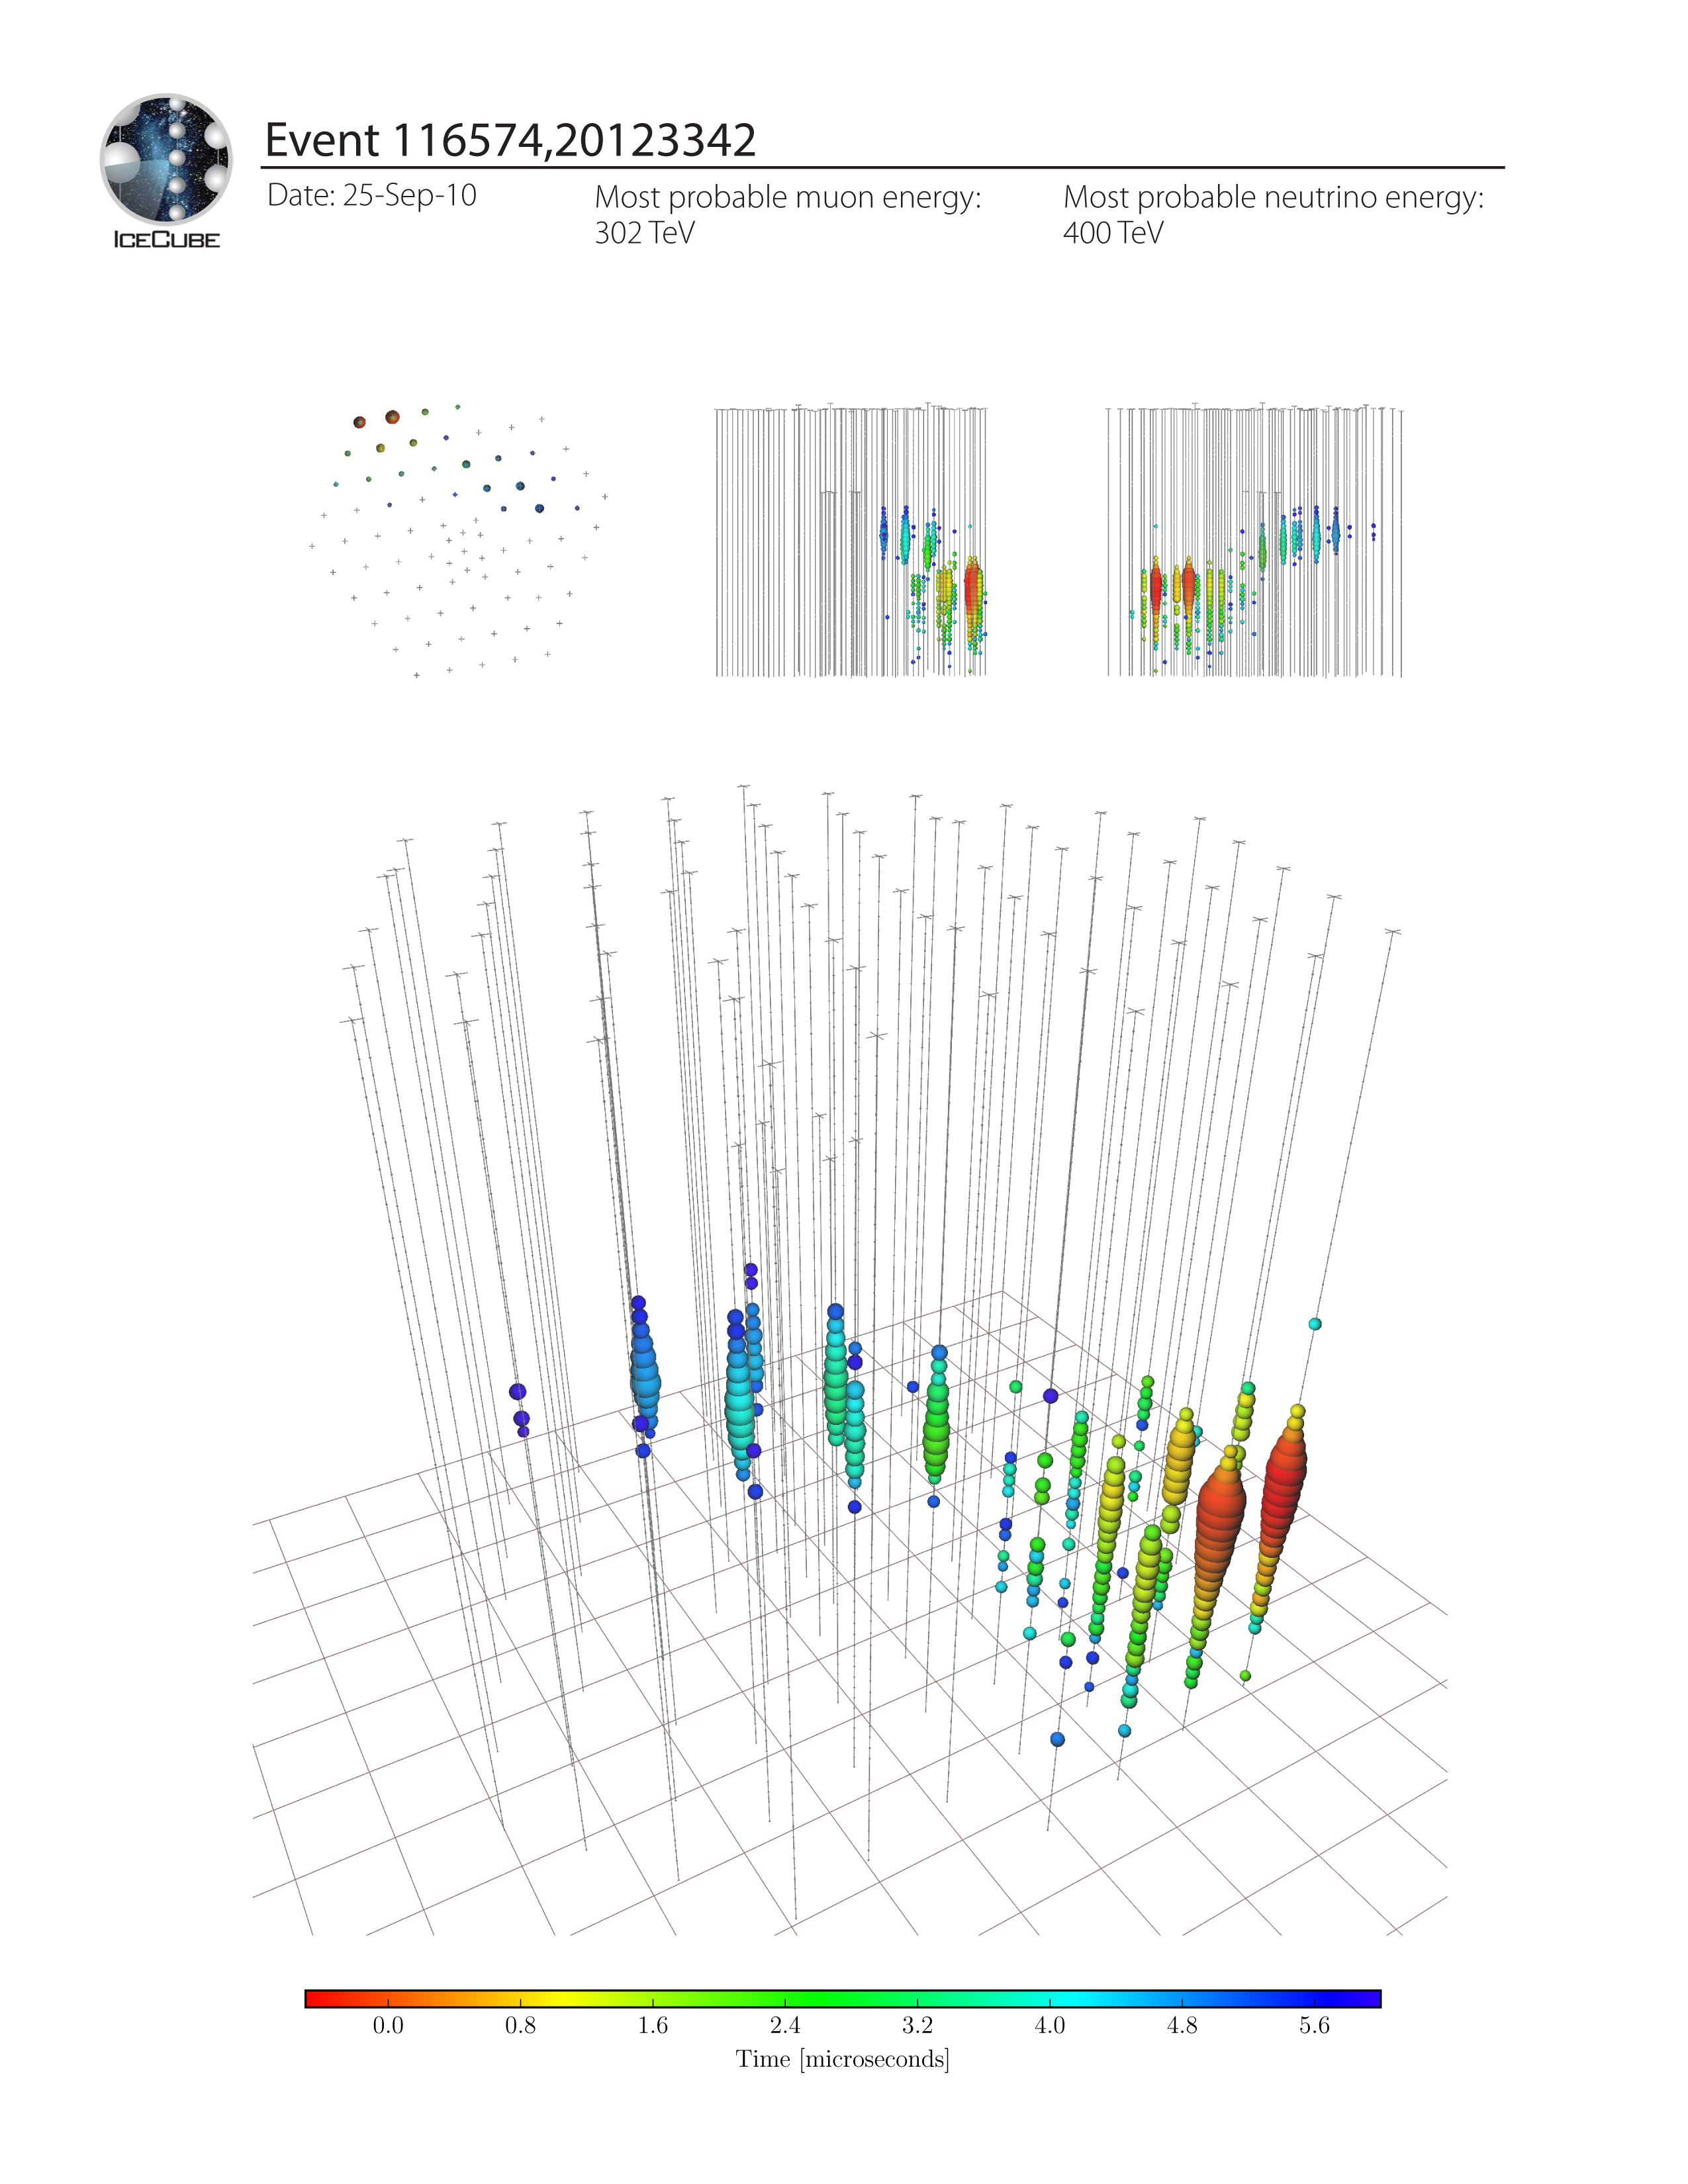
\includegraphics[scale=0.43]{images/track.png} \\
    \textit{[Fig. 1]}
\end{center}
Das $\nu_\mu \,/\, \overline{\nu}_\mu$ hinterlässt Myonen. Wenn die Myonen durch den Detektor passieren
hinterlassen sie Cherenkov-Licht, da sie in Relation zur Lichtgeschwindigkeit im Eis sich schneller fortbewegen.
Da wie in \textit{[Fig 1]} ersichtlich wird das eine Spursignatur hinterlässt ist es einfach zu bestimmen aus
welcher Richtung das Myon kommt. Es wird eine Lineare Regression angefertigt. Das von den optischen Sensoren aufgenomme
Licht steht in Korrelation zur Myonenenergie.\cite{Halzen2012} \cite{Martinez2016}
\newpage

\subsection{Kaskadensignatur\,/\,$e$-Signatur}
\begin{center}
    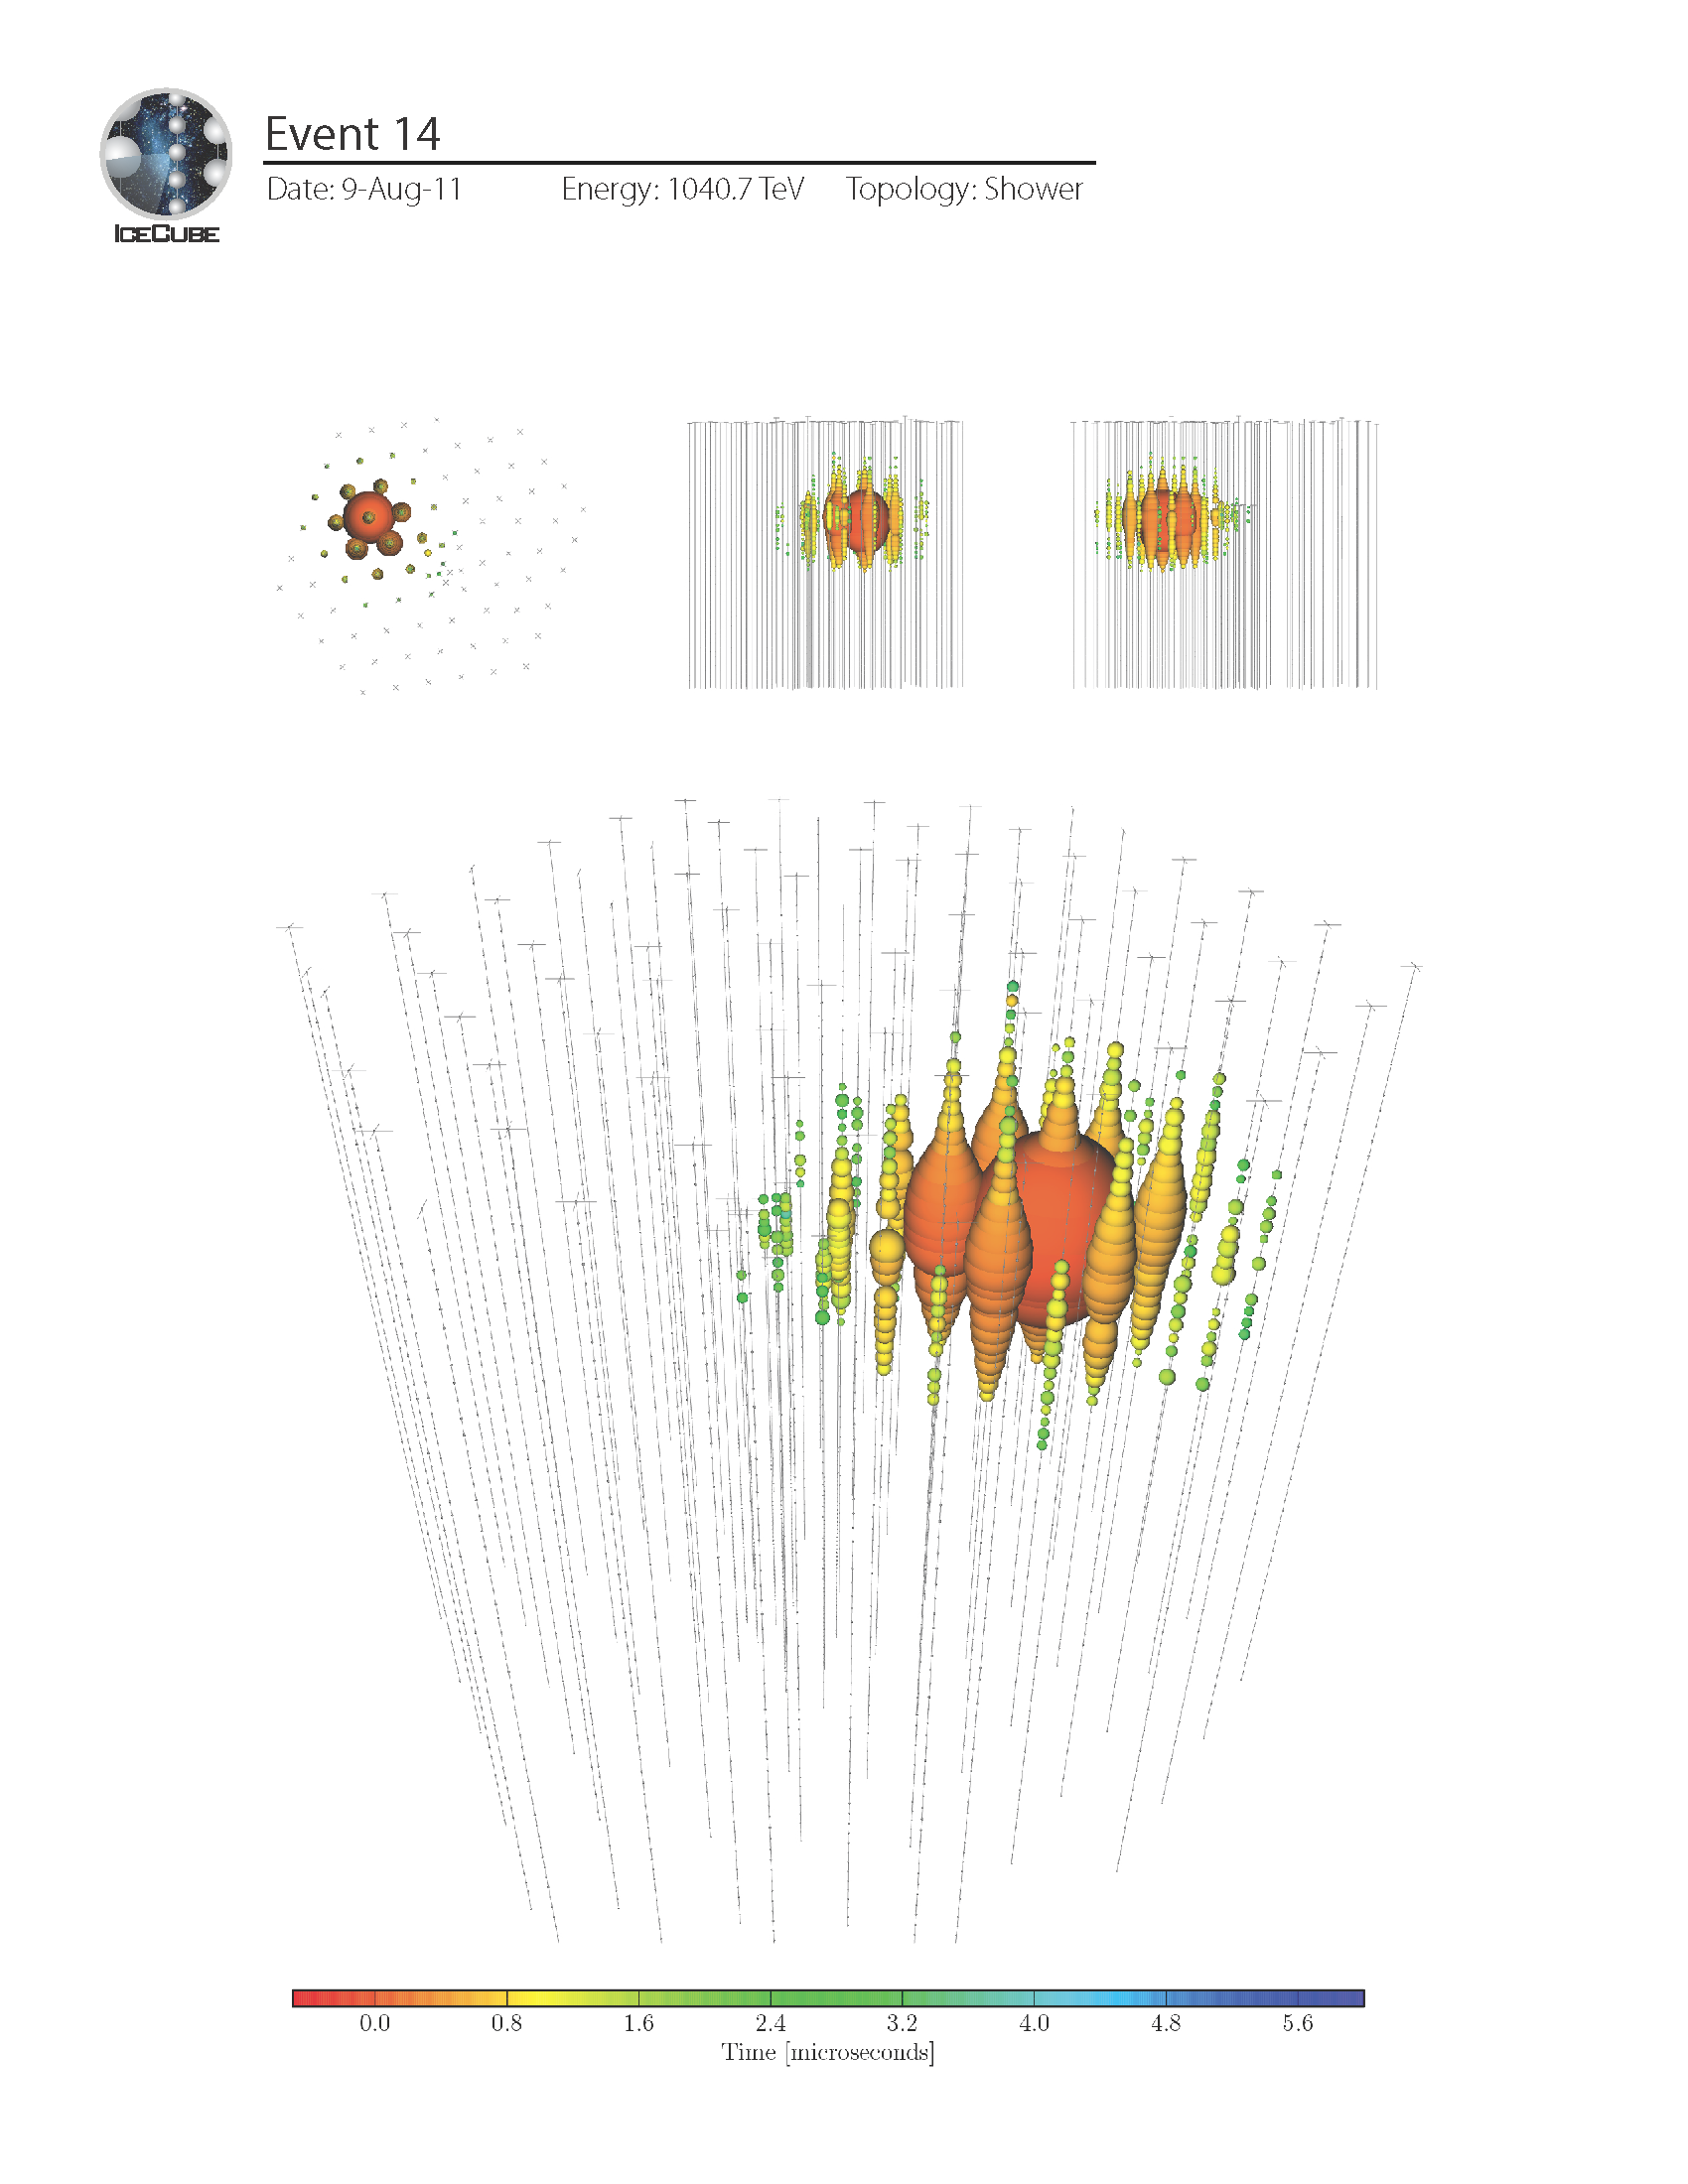
\includegraphics[scale=0.45]{images/cascade.png} \\
    \textit{[Fig. 2]}
\end{center}
Das $\nu_e \,/\, \overline{\nu}_e$ hinterlässt eine Kaskade. Wenn es im Detektor wechselwirkt hinterlässt es einen Teilchenschauer.
Die Teilchen hinterlassen Cherenkov-Licht,  da sie in Relation zur Lichtgeschwindigkeit im Eis sich schneller fortbewegen.
Wie man in \textit{[Fig. 2]} entsteht dadurch eine kugelförmige Signatur. Das von den optischen Sensoren aufgenomme
Licht steht in Korrelation zum der freigegeben Energie durch die Wechselwirkung mit dem Detektor. \cite{Halzen2012}
\newpage

\subsection{Double-Bang-Signatur\,/\,$\tau$-Signatur}
\begin{center}
    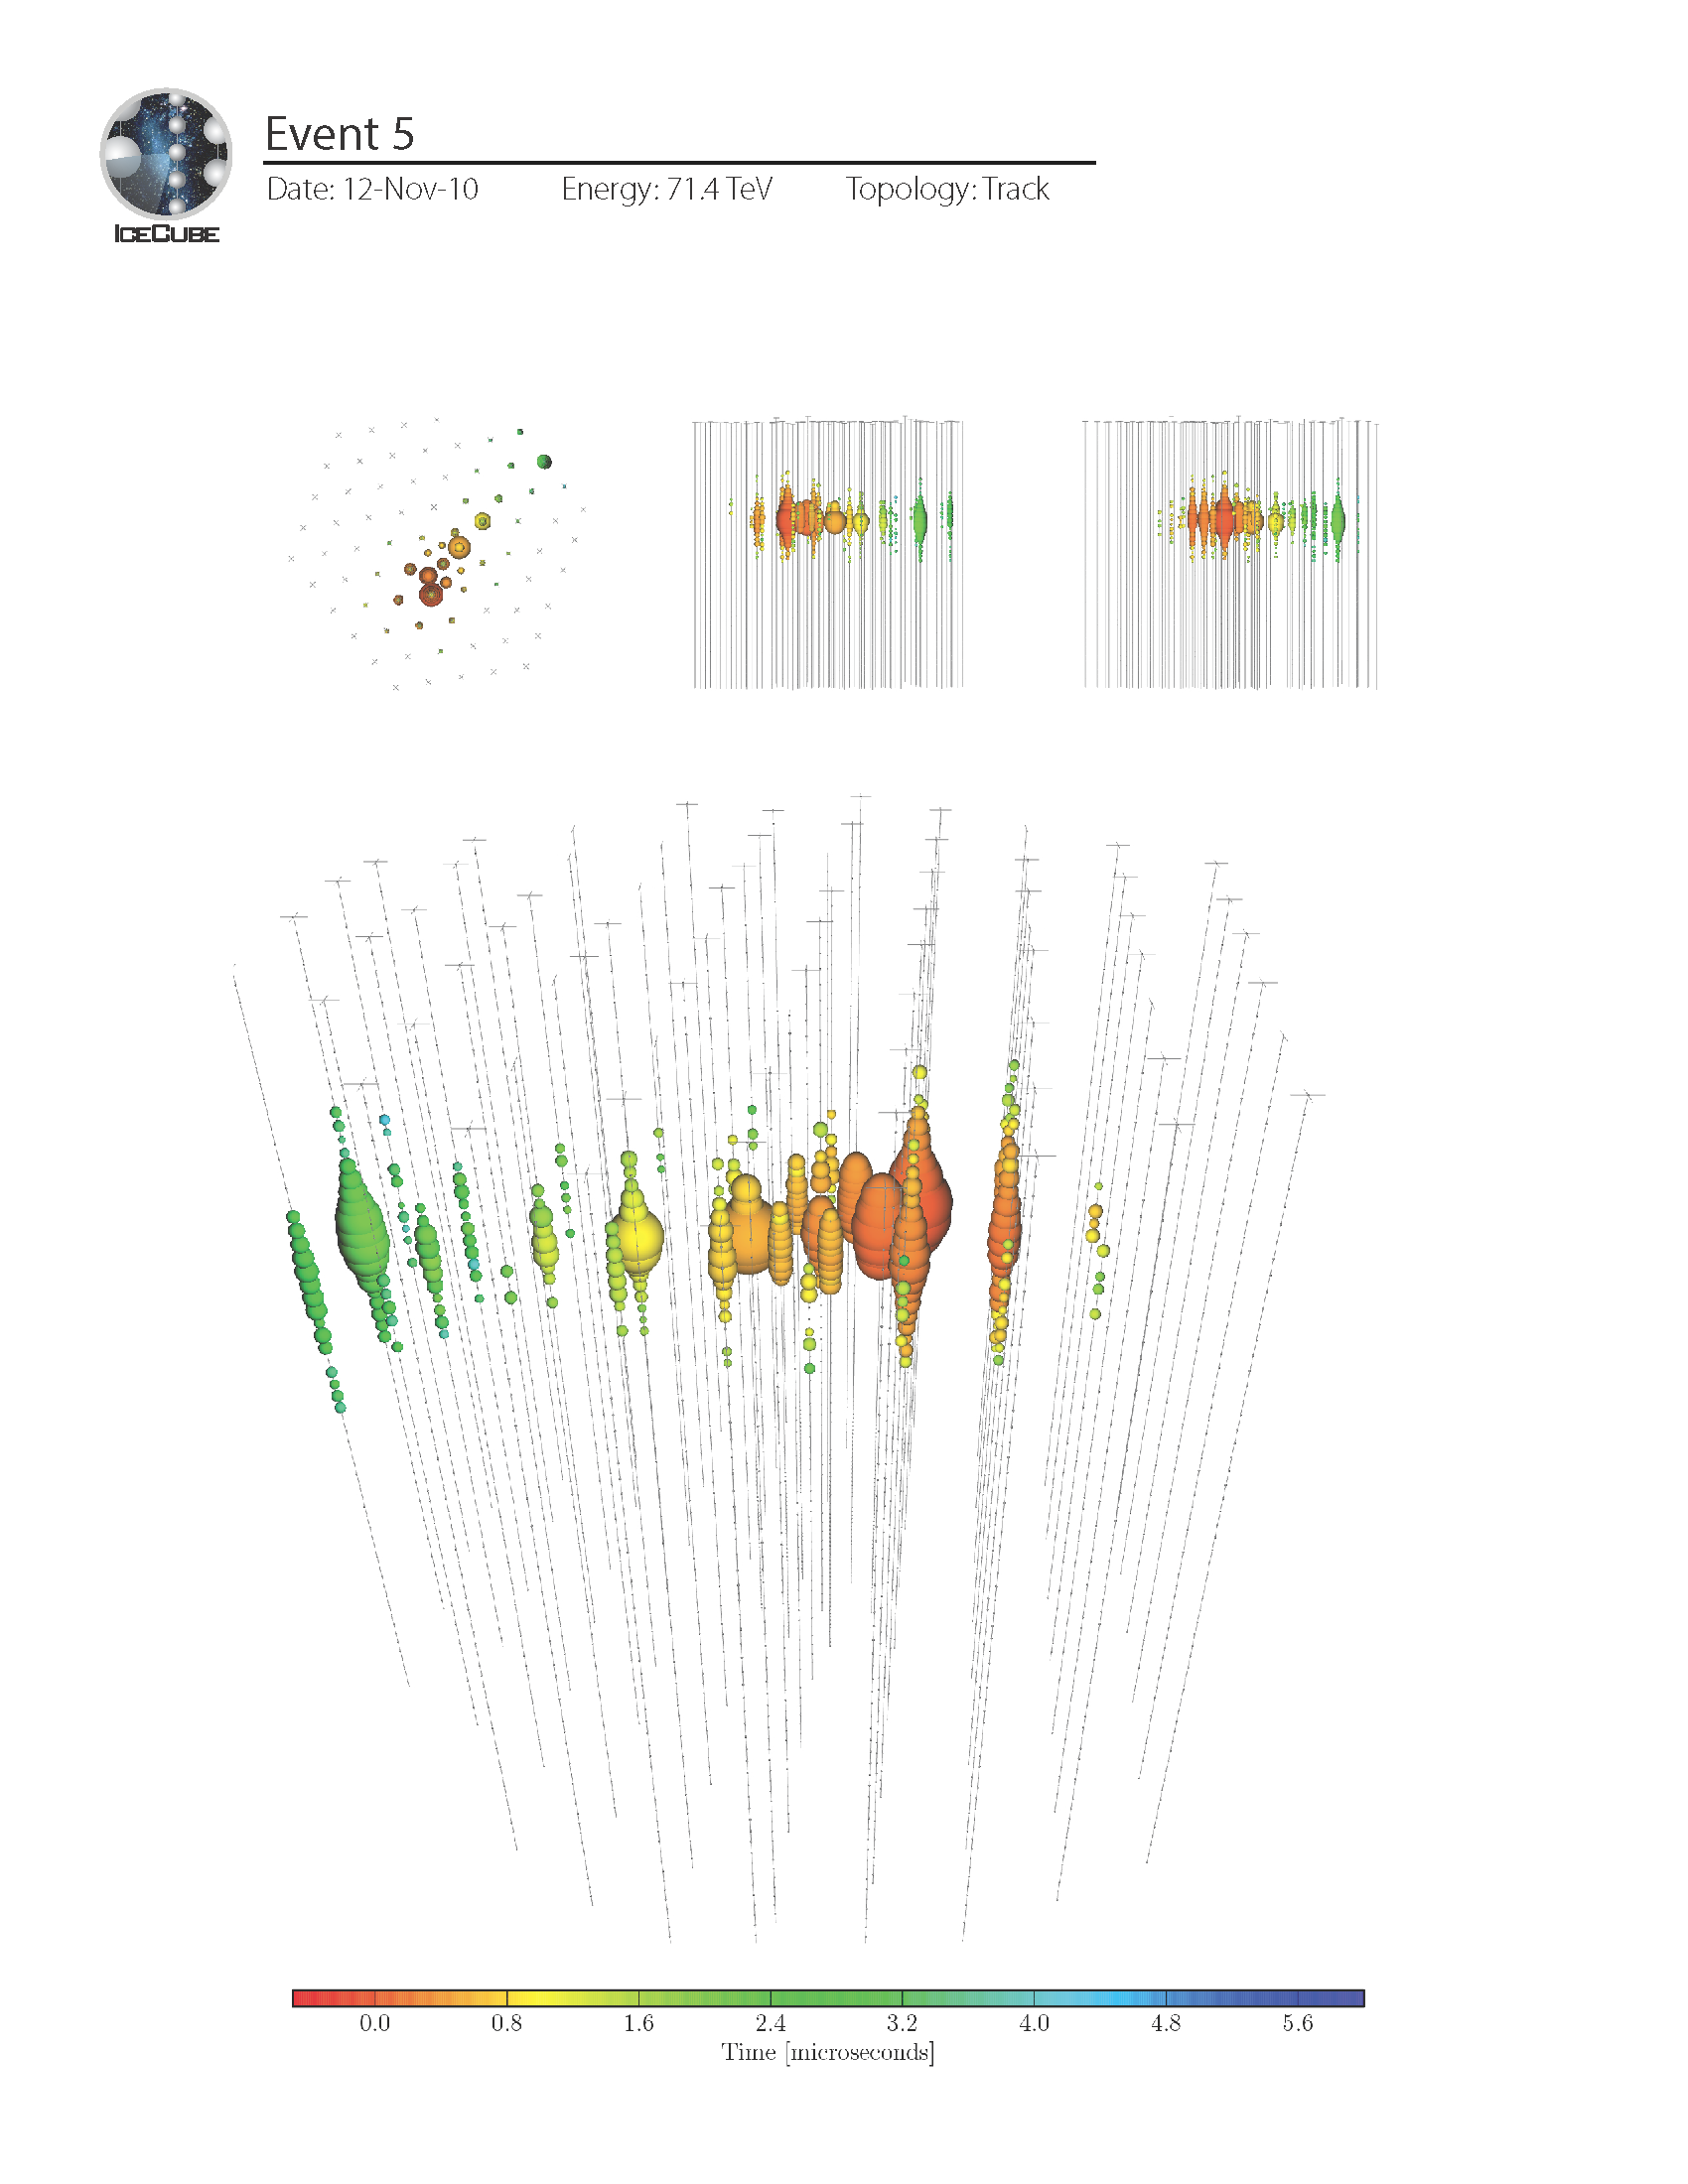
\includegraphics[scale=0.45]{images/doublebang.png} \\
    \textit{[Fig. 3]}
\end{center}
Bei der Double-Bang-Signatur hat ein $\nu_\tau \,/\, \overline{\nu}_\tau$ mit einer Energie über 1 PeV eine erste Kaskade verursacht.
Bei dieser Kaskade entsteht ein $\tau$, welches dann zerfällt und eine zweite Kaskade verursacht.
Wie man in \textit{[Fig. 3]} entstehen dann 2 Kaskaden. Einmal gibt es eine rote Kaskade und dann eine grüne Kaskade.
Die rote Kaskade ist die erste Kaskade und ist dann mit der grünen zweite Kaskade verbunden. Diese Signatur ähnelt
sehr der Spursignatur, man kann sie aber an der ungleichmäßigen Größe der Signale unterscheiden. \cite{Halzen2012}